%!TEX root = ../dokumentation.tex

\chapter{Architektur}\label{cha:Architektur}
~\cite{mvc1}
\section{Architektur Konzept}\label{sec:Architektur Konzept}
Wie in Abbildung ~\ref{fig:Architektur_grob} zu sehen ist, besteht das System im Kern aus 3 Komponenten. Die Drohne, das \acs{XDK} sowie das Tablet sind alle mit dem \acs{WLAN} der Drohne verbunden. Über dieses läuft dann die komplette Kommunikation zwischen den einzelnen Komponenten ab. Die App kommuniziert über das \acs{DJI}-\acs{SDK} mit der Drohne, das \acs{XDK} baut eine UDP-Verbindung zur App auf, über die es die gemessenen Sensordaten schicken kann.
\begin{figure}[H]
	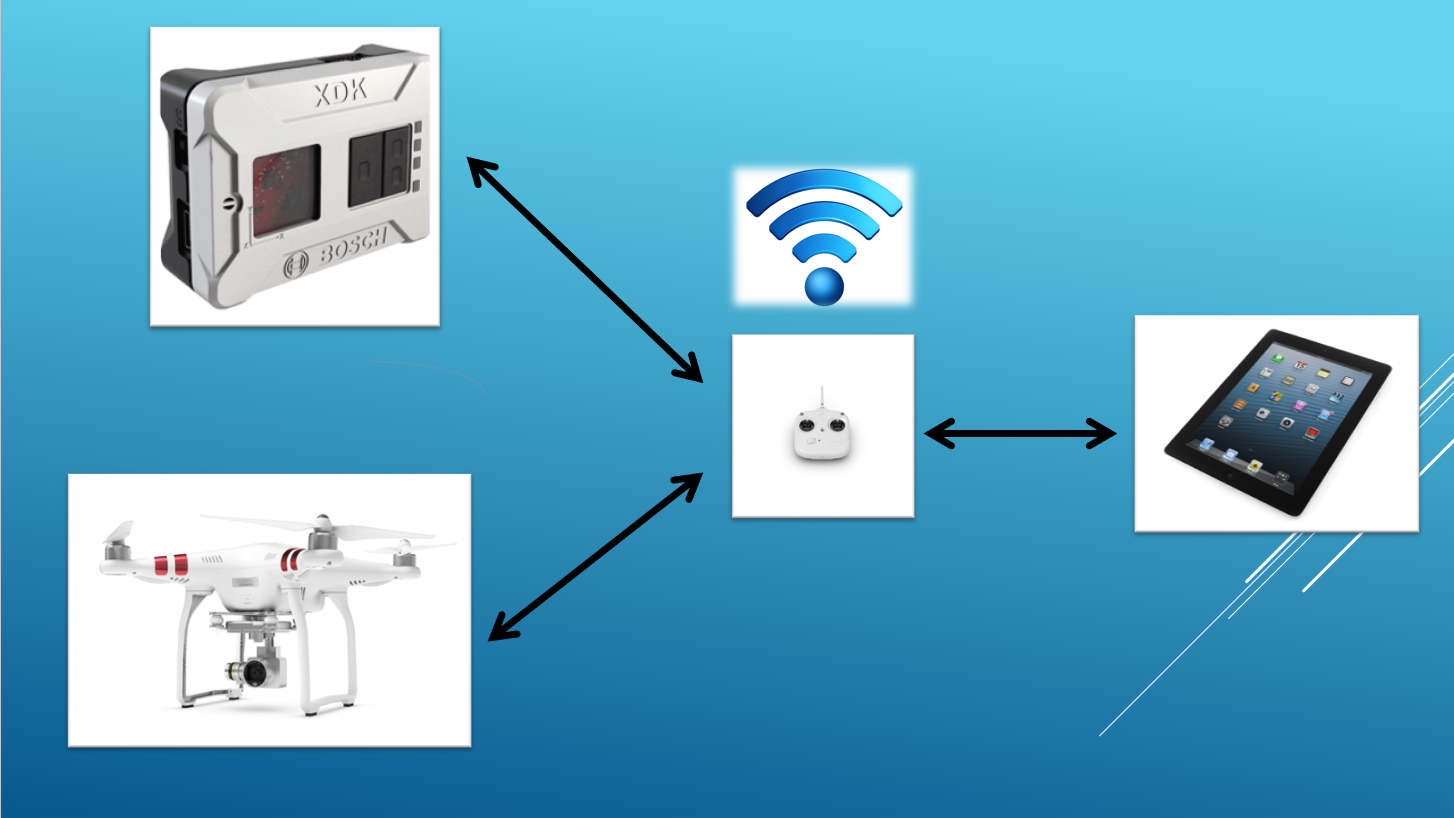
\includegraphics[width=\textwidth]{images/Architektur_grob.png}	
	\caption{Architektur allgemein}
	\label{fig:Architektur_grob}
\end{figure}

\section{Lesen der Sensordaten}\label{sec:Lesen der Sensordaten}
Abbildung ~\ref{fig:Architektur_fein} zeigt schematisch das Auslesen der Sensordaten am \acs{XDK}. Das \acs{XDK} ist mit dem dazu passenden Extension Board direkt über eine serielle Schnittstelle verbunden, über die es die Messwerte der externen Sensoren empfängt. 
\newline
Für die analogen Sensoren werden prinzipiell deren Spannungspegel am Ausgang auf einen Multiplexer geleitet, der in Abhängigkeit des Signales vom Extension Board entscheidet, welcher Sensor-Ausgang auf den Ausgang des Multiplexers übertragen wird. Die Ansteuerung des Multiplexers erfolgt auf Seiten der Software auf dem \acs{XDK}. Darin wird festgelegt, wie genau die \acs{GPIO}-Pins des Extension-Boards zu beschalten sind. Abschließend wird dann der Wert am Ausgang des Multiplexers vom Analog-Digital-Wandler des Extension Boards erfasst und an das \acs{XDK} übermittelt.
\newline
Die Messwerte des Feinstaub-Sensors SDS011 können lediglich über \acs{UART} erfasst werden. Aus diesem Grund wird der Sensor nicht mit dem Multiplexer verbunden, sondern direkt, beziehungsweise nach Anpassung des Spannungs-Pegels, mit dem Extension Board verbunden. In der Software des \acs{XDK} lässt sich dann konfigurieren, dass die mit dem Sensor verbundenen Pins für \acs{UART} genutzt werden sollen, womit die Messwerte direkt in digitaler Form am XDK erfasst werden können.
\newline
Aufgrund dessen, dass der Feinstaub-Sensor die gemessenen Daten höchstens im Sekundentakt per UART übermitteln kann, ist die maximale Messdichte ebenfalls auf 1 Messung pro Sekunde beschränkt. Damit die 5 analogen Sensoren auch mindestens einmal in diesem Intervall ihre Daten an das XDK weitergeben, werden die \acs{GPIO}-Pins von der Software alle 100ms geändert, sodass immer ein anderer Sensor am Analog-Digital-Wandler anliegt. 
\newline
Sind nun in einer Sekunde alle Daten einmal gemessen, so sendet das \acs{XDK} diese sofort per \acs{UDP} über das \acs{WLAN} der Drohne an die iOS-Applikation, wo die Messdaten dann visualisiert werden können.

\begin{figure}[H]	
	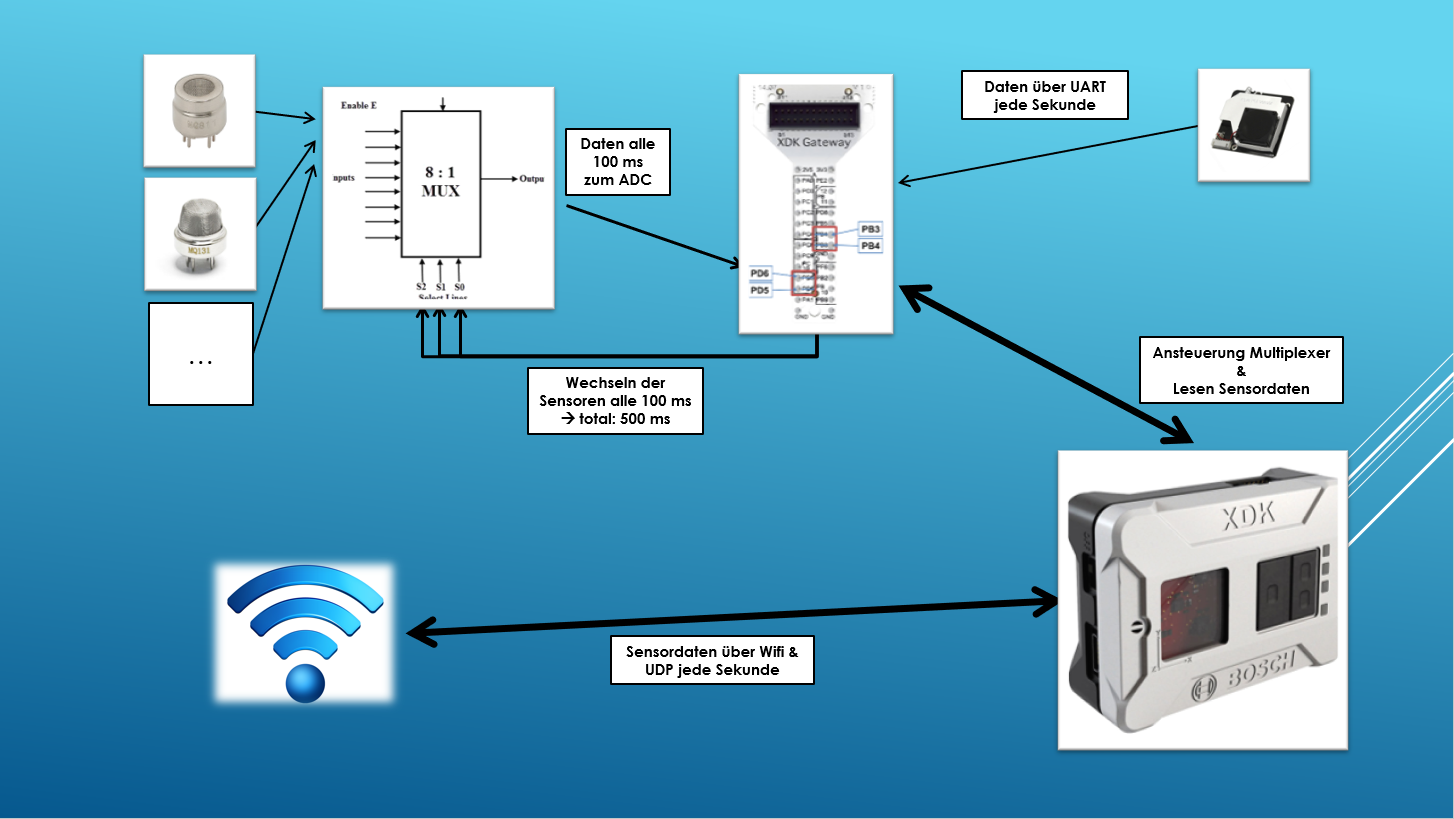
\includegraphics[width=\textwidth]{images/Architektur_fein.png}	
	\caption{Architektur Sensorik}
	\label{fig:Architektur_fein}
\end{figure}

Wie wir basierend auf der vorangegangenen Tabelle erkennen können, liefert kein Sensor einen Pegel von 2,5V, wie er vom \acs{XDK} benötigt wird. Damit die von den Sensoren gelieferten Daten nun also verarbeitet werden können, müssen die Pegel angepasst werden. Um dies zu erreichen, wird ein Operationsverstärker verwendet, der die Ausgangsspannung um die Hälfte reduziert. Näheres zu diesem Prozess in Abschnitt ~\ref{subsec:Operationsverstärker}.
Neben der Anpassung der Pegel ist noch ein weiterer Schritt erforderlich, um die analogen Sensordaten lesen zu können. Bedingt dadurch, dass 5 analoge Sensoren auszuwerten sind und dafür lediglich 2 Pins verfügbar sind, welche als \acs{ADC} genutzt werden können, müssen mehrere der Sensoren mit einem \acs{ADC} gemessen werden. Um dies zu ermöglichen, werden die Sensordaten mit Hilfe eines Multiplexers in verschiedenen Zeitschlitzen übermittelt. Um den Multiplexer anzusteuern werden dabei die \acs{GPIO}-Pins des \acs{XDK} verwendet. Die genaue Beschreibung hierzu lässt sich in Abschnitt ~\ref{subsec:Multiplexer} finden.

Neben den 5 analogen Sensoren muss auch das Signal des Feinstaub-Sensors angepasst werden, welcher die Daten seriell über \acs{UART} mit 3,3V übermittelt. Um dieses Signal auf die erforderlichen 2,5V umzuwandeln, wird ein Pegelwandler verwendet, der diskrete Pegel konvertieren kann. Dies wird in Abschnitt ~\ref{subsec:Pegelwandler} näher beschrieben.

\section{Schaltungsdesign}\label{sec:Schaltungsdesign}
Da die Sensoren aus Tabelle ~\ref{tab:Sensoren} Ausgangs-Spannungen zwischen 0V und 5V liefern, müssen diese Spannungen noch umgewandelt werden, bevor sie mit dem Extension Board und somit dem XDK verbunden werden dürfen. Aus diesem Grund werden mehrere Pegel-Wandler und Operationsverstärker eingesetzt, damit die einzelnen Komponenten kompatibel werden.
\newline
In diesem Abschnitt wird nun näher auf das konkrete Schaltungs-Design eingegangen, wie die Bauteile elektrisch miteinander verbunden sind und wie die Spannungen umgewandelt werden, sodass die einzelnen Komponenten miteinander kommunizieren können. Ein Überblick über das gesamte Schaltungslayout lässt sich im Anhang in Abschnit ~\ref{label} finden.
\newline
Die gezeigten Schaltungs-Layouts und die dabei verwendeten Komponenten sind mit Hilfe der gratis \acf{CAD}-Software PCBWeb entworfen worden, die sowohl zum Entwurf schematischer Schaltpläne, als auch zur Erstellung von \acf{PCB}-Layouts verwendet werden kann.
\subsection{Extension-Board}\label{subsec:Extension-Board}
\begin{figure}[H]
	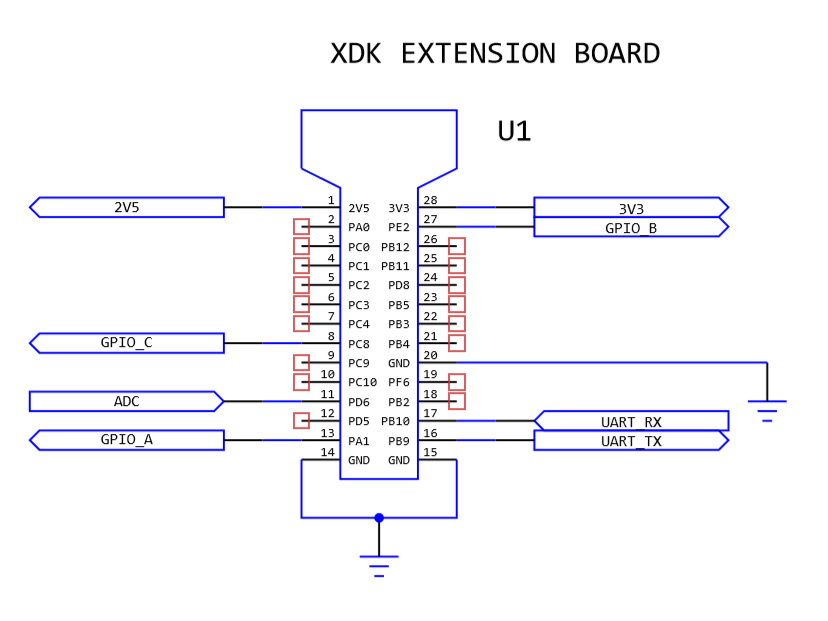
\includegraphics[width=\textwidth]{images/Layout_XDK.png}	
	\caption{Layout Extension-Board}
	\label{fig:Layout_ExtensionBoard}
\end{figure}
Abbildung ~\ref{fig:Layout_ExtensionBoard} zeigt ganz konkret die Beschaltung des Boards und wie die angeschlossenen Pins verwendet werden. Die Pins 1 und 28 dienen als Spannungsquelle für alle Komponenten, die Spannungen von 2,5V oder 3,3V benötigen. 
\newline
Die Pins PA1, PE2 sowie PC8 werden als \acs{GPIO}-Pins benutzt, mit denen der Multiplexer angesteuert wird.
\newline
PD6 ist konfiguriert, um als Analog-Digital-Wandler die Spannungen der analogen Sensoren zu digitalisieren. Dazu wird er nach einer Anpassung des Spannungspegels mit dem Multiplexer verbunden.
\newline
Die beiden Pins PB9 und PB10 sind für \acs{UART} konfiguriert und werden mit letztlich mit dem Feinstaub-Sensor SDS011 verbunden.
\subsection{Multiplexer}\label{subsec:Multiplexer}
\begin{figure}[H]
	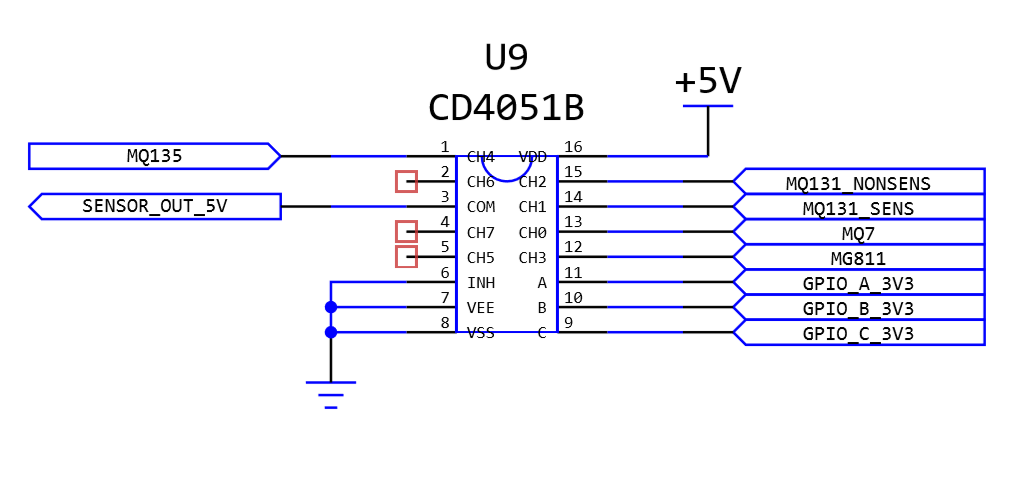
\includegraphics[width=\textwidth]{images/Layout_Multiplexer.png}	
	\caption{Layout Multiplexer}
	\label{fig:Layout_Multiplexer}
\end{figure}
Damit der Multiplexer die Spannungs-Werte der Sensoren auf den Ausgang durchschalten kann, benötigt er an den Steuerungs-Eingängen A, B und C Spannungen von mindestens 3,3V. Aus diesem Grund können nicht einfach die \acs{GPIO}-Pins des Extension-Boards direkt mit dem Multiplexer verbunden werden, da diese lediglich 2,5V liefern. Damit diese Pegel angepasst werden, werden die \acs{GPIO}-Pins zunächst mit einem Pegelwandler verbunden, wie in Abbildung ~\ref{fig:Layout_LevelShifter} zu sehen ist.
\newline
Wenn somit die Steuerung des Multiplexers funktioniert, wird abhängig von der Beschaltung der Pins A, B und C der Ausgang COM auf den passenden Eingangskanal durchgeschaltet. Tabelle ~\ref{tab:MultiplexerLogic} zeigt die logischen Verknüpfungen.
\begin{table}[H]
	\begin{center}
			\begin{tabular}{|c|c|c|c|}
				\hline
				A & B & C & Output (Channel)  \\ \hline \hline
				
				0 & 0 & 0 & 0 \\ \hline 
				0 & 0 & 1 & 1 \\ \hline 
				0 & 1 & 0 & 2 \\ \hline 
				0 & 1 & 1 & 3 \\ \hline 
				1 & 0 & 0 & 4 \\ \hline 
				1 & 0 & 1 & 5 \\ \hline 
				1 & 1 & 0 & 6 \\ \hline 
				1 & 1 & 1 & 7 \\ \hline 							
			\end{tabular}
	\end{center}
	\caption{Logische Ansteuerung Multiplexer}
	\label{tab:MultiplexerLogic}
\end{table}
Ist nun ein bestimmter Eingangskanal auf den Ausgang durchgeschaltet, so kann das Signal trotzdem noch nicht mit dem \acs{ADC} verbunden werden, da die Spannungswerte des Signals zwischen 0V und 5V liegen können. Da das XDK nur Spannungen bis zu 2,5V verträgt, muss die Spannung auf diesen Bereich umgewandelt werden. Wie dies zu erreichen ist, wird in Abschnitt ~\ref{subsec:Operationsverstärker} näher erläutert.
\subsection{Pegelwandler}\label{subsec:Pegelwandler}
\begin{figure}[H]
	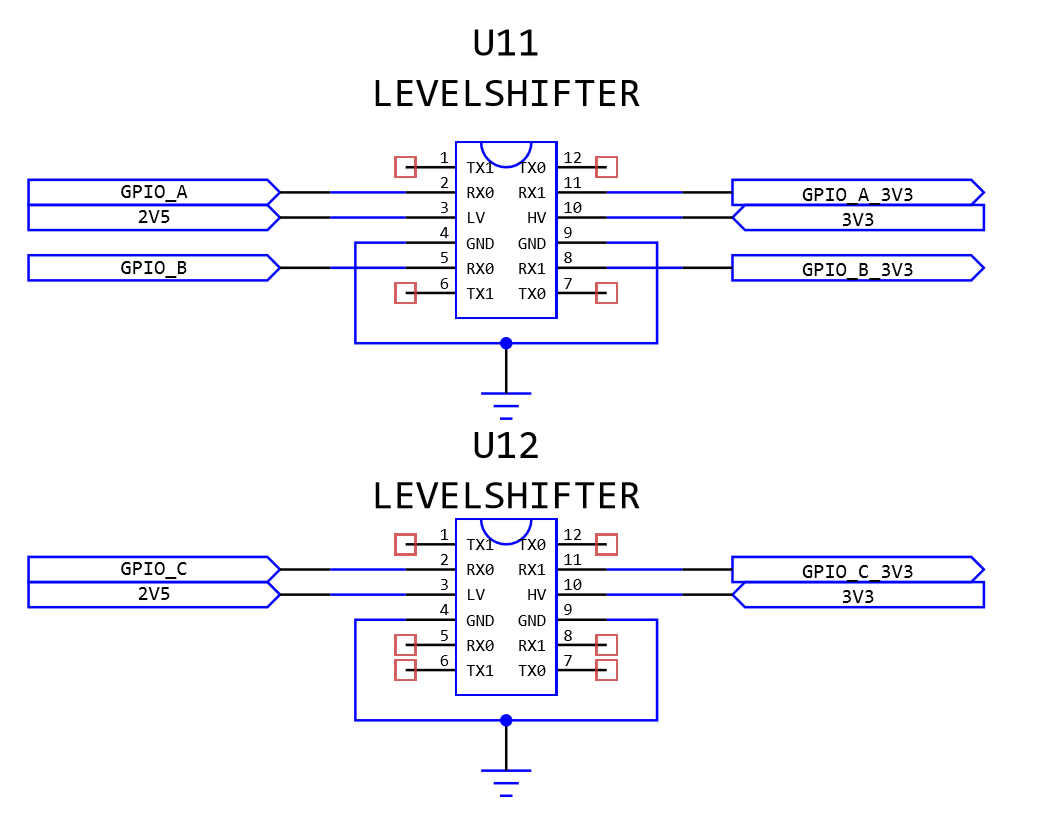
\includegraphics[width=\textwidth]{images/Layout_LevelShifter.png}	
	\caption{Layout Pegelwandler}
	\label{fig:Layout_LevelShifter}
\end{figure}
Wie bereits zuvor erwähnt werden die beiden Pegelwandler benutzt, um die Spannung der von den \acs{GPIO}-Pins eingehenden Signale auf 3,3V anzuheben, damit der Multiplexer diese verarbeiten kann.
\subsection{Operationsverstärker}\label{subsec:Operationsverstärker}
Wie im Abschnitt ~\ref{subsec:Multiplexer} erwähnt, muss das Ausgangssignal des Multiplexers aus dem Intervall von 0V bis 5V in das Intervall von 0V bis 2,5V konvertiert werden. Dies geschieht mittels eines Operationsverstärkers und der dazugehörigen Grundschaltung des invertierenden Verstärkers, welche in Abbildung ~\ref{fig:InvertierenderVerstärker} zu sehen ist.
\begin{figure}[H]
	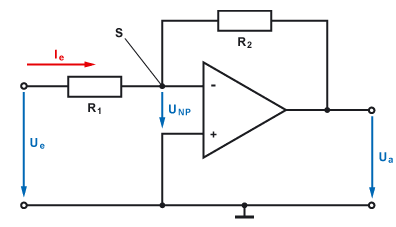
\includegraphics{images/InvertierenderVerstaerker.png}	
	\caption{Invertierender Verstärker}
	\label{fig:InvertierenderVerstaerker}
\end{figure}
Laut der Grundgleichung des invertierenden Verstärkers wird der Verstärkungsfaktor V berechnet mit:
\[ V_u = \frac{U_a}{U_e} = -\frac{R_2}{R_1} \]
Um nun eine Dämpfung um den Faktor 2 zu erhalten, beschalten wir einen ersten Operationsverstärker mit \(R_1 = 20K\Omega\) und \(R_2 = 10K\Omega\). Da dadurch das Signal allerdings im Intervall von -2,5V bis 0V liegt, wird ein weiterer Operationsverstärker damit beschaltet, der die Wiederstände \(R_3 = 10K\Omega\) und \(R_4 = 10K\Omega\) besitzt, wodurch das Signal erneut invertiert wird und es somit im korrekten Intervall erscheint. 
\newline
Diese schematische Beschaltung ist in Abbildung ~\ref{fig:Layout_OP} zu erkennen.
\begin{figure}[H]
	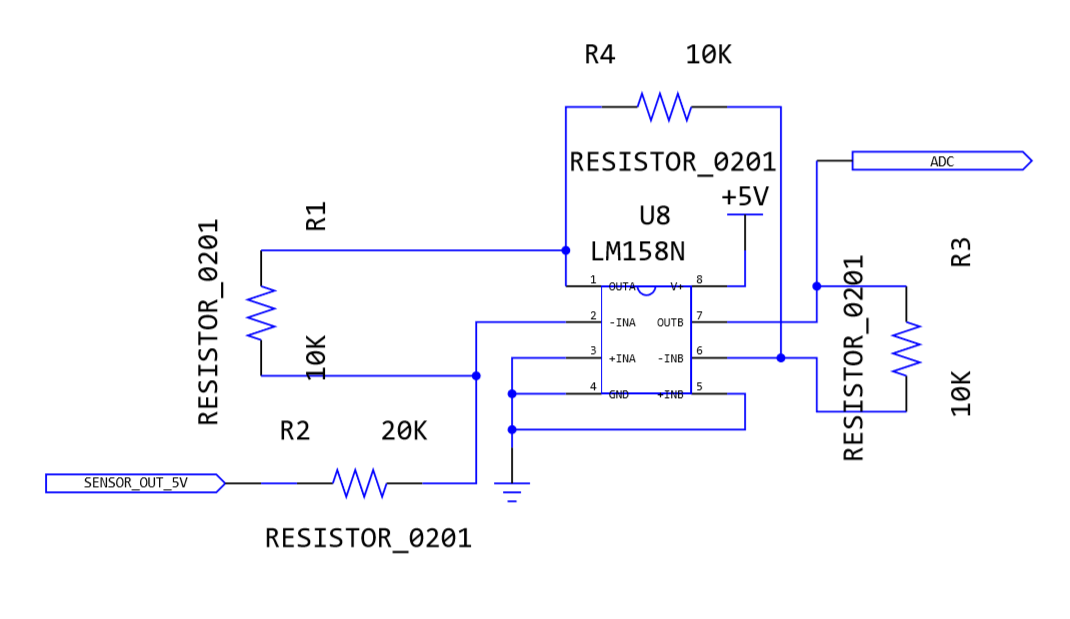
\includegraphics[width=\textwidth]{images/Layout_OP.png}	
	\caption{Layout Operationsverstärker}
	\label{fig:Layout_OP}
\end{figure}
\subsection{Feinstaub-Sensor}\label{subsec:Feinstaub-Sensor}
Abbildung ~\ref{fig:Layout_SDS011} zeigt die Beschaltung des Feinstaub-Sensors. Man kann erkennen, dass auch hier die Signale des Sensors zunächst auf einen Pegelwandler geschickt werden, damit dieser die Spannungspegel von 3,3V auf 2,5V umwandelt. Nach der Umwandlung werden die daraus resultierenden Signale direkt mit den entsprechenden Pins am \acs{XDK} Extension Board verbunden, an denen die digitalisierten Messwerte über \acs{UART} ausgelesen werden.
\begin{figure}[H]
	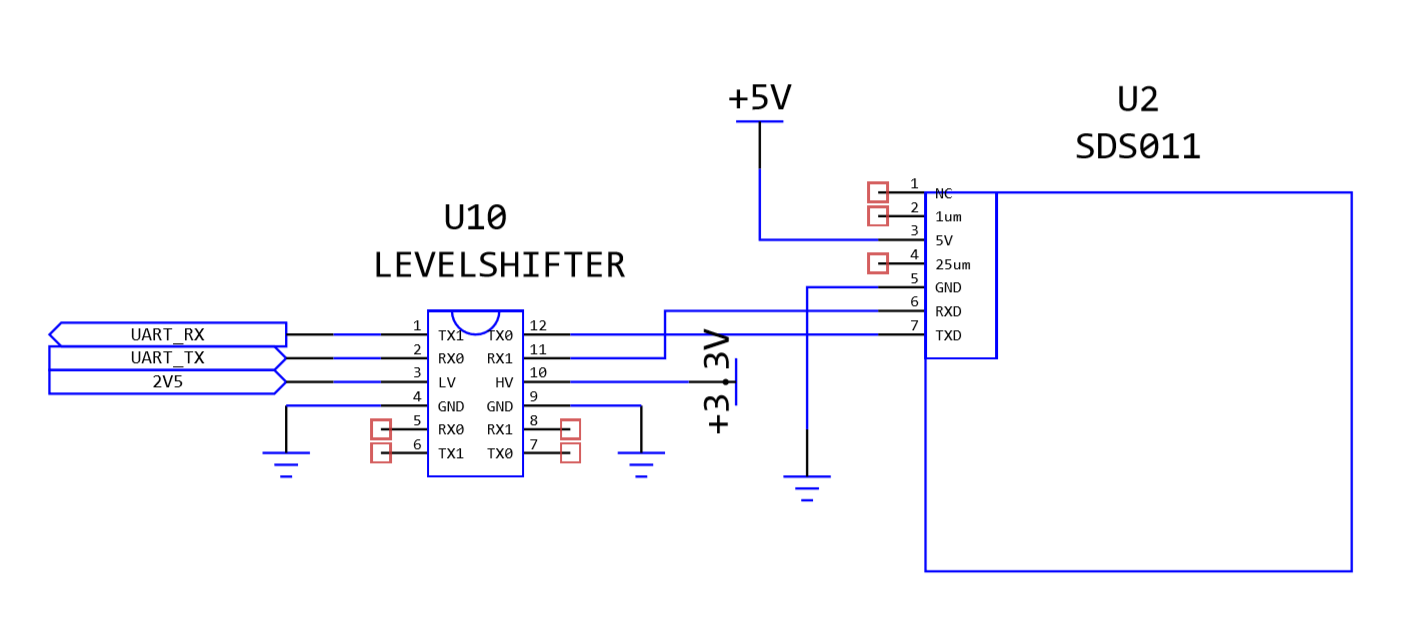
\includegraphics[width=\textwidth]{images/Layout_SDS011.png}	
	\caption{Layout Feinstaub-Sensor}
	\label{fig:Layout_SDS011}
\end{figure}
\subsection{Layout analoger Sensor}\label{subsec:Layout analoger Sensor}
Zum Abschluss der Schaltungs-Layouts zeigt Abbildung ~\ref{fig:Layout_Sensor_Example} eine beispielhafte Beschaltung eines der analogen Sensoren. Da diese bei allen anderen Sensoren praktisch gleich aussieht, wird hier nur die Abbildung des MQ7-Sensors zur Veranschaulichung dargestellt. Die vollständigen Layouts der Sensoren finden sich im Anhang in Abschnitt ~\ref{label}.
\begin{figure}[H]
	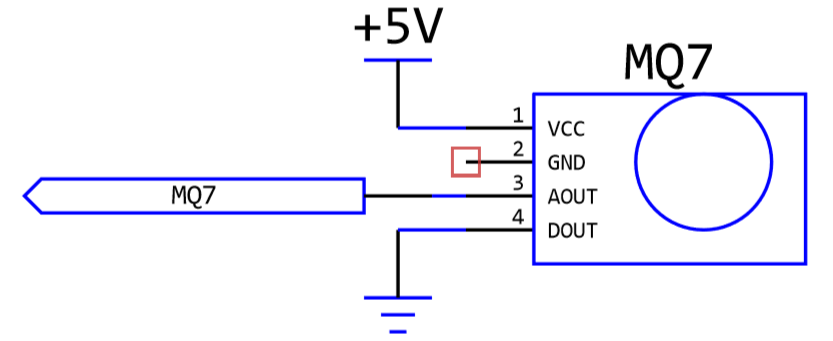
\includegraphics[width=8cm]{images/Layout_Sensor_Example.png}	
	\caption{Layout analoger Sensor}
	\label{fig:Layout_Sensor_Example}
\end{figure}